\chapter{A New Approach}
\label{chap:diagrams}

In your thesis you will be expected to present some sort of new
treatment of your subject.  Since this may well involve the use
of diagrams, I will take this opportunity to explain the use of
``floating'' figures and including graphics files.

\section{Floats}
Because \LaTeX\ forces the writer to concentrate on content rather
than formatting, you may never be sure where pages will break or where
figures will be placed.  \LaTeX\ uses a system of ``Floats'' for
figures and tables which ensure that they will be put in the most
convenient place.

\begin{figure}[htb]
\begin{center}
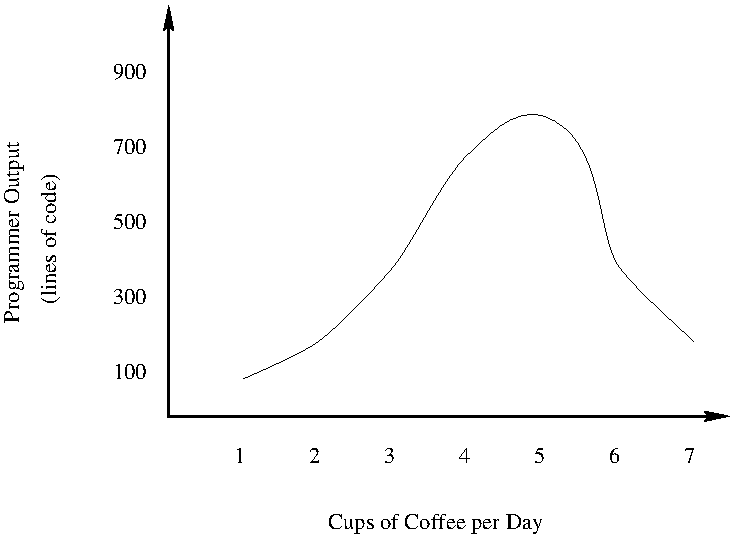
\includegraphics[height = 110mm]{graph1.pdf}
\caption[An example of a floating figure.]{An example of a floating
         figure.  Captions for diagrams generally go {\em underneath} the
         figure itself.}
\label{fig:graph1}
\end{center}
\end{figure}

Figure~\ref{fig:graph1} is an example of a floating figure.  Note that
even though the code for it is placed before this paragraph, the
figure is appearing after this text; it has been ``floated'' into a
more convenient place. The code for the figure looks like this: \par
\linespread{1} \small
\begin{quote}
\begin{verbatim}
\begin{figure}[htb]
\begin{center}
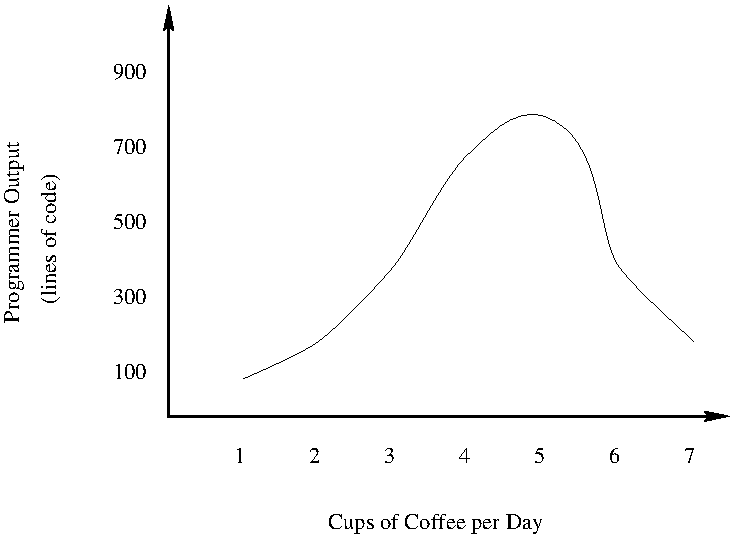
\includegraphics[height = 110mm]{graph1.pdf}
\caption[An example of a floating figure.]{An example of a floating
         figure.  Captions for diagrams generally go {\em underneath}
         the figure itself.}
\label{fig:graph1}
\end{center}
\end{figure}
\end{verbatim}
\end{quote}
\linespread{1.3} \normalsize

Both width and height can be scaled using the optional part of the
\small
\verb|\includegraphics| \normalsize
command.  If you scale just one or the
other, the aspect ratio will be maintained.  If you try to scale
both, you run the risk of your picture being ``squished''.

Under Pdflatex, you may use GIF, JPEG, TIFF, PNG, or PDF graphics.  All
will work the same way.  Bear in mind that if you are drawing a {\em
diagram}, it is best to use a vector format that will scale (e.g.\
as PDF), whereas photographs and screenshots may as well be in JPEG or
PNG format.

The [htb] part gives \LaTeX\ the options you want to use to try placing
the figure.  First, it will try to place the float at the exact
position in the text.  Next, it will try to place it at the top, then
bottom of the current page.  Finally, if [p] is also specified, 
it will try to place it on a page dedicated only to floats.  The order
of [htb] after \verb|\begin{figure}| is irrelevant---it will always
try to place figures in this order.  The options just tell it
{\em what} it is allowed to try, not the order it tries it.

The caption has two parts: the part inside the square brackets  is
what appears on your List of Figures page, and the part inside the
braces is what appears under the figure itself.

The \verb|\label| part  gives you a label so you can reference your
figure. The command \verb|\ref{fig:graph1}| will be replaced in your
text by the actual number of the figure;
e.g. \verb|Figure~\ref{fig:graph1}| will come out as ``Figure 3.1''.
For this number to be correct, the \verb|\label| part {\em must} come
{\em after} the \verb|\caption| part.  Also don't forget that if you
have a figure with a caption you are required to refer to it somewhere
in your text.

Here is the figure again;
this time we will make \LaTeX\ try {\em really hard} to put the figure
right {\em here}.

\begin{figure}[!h]
\begin{center}
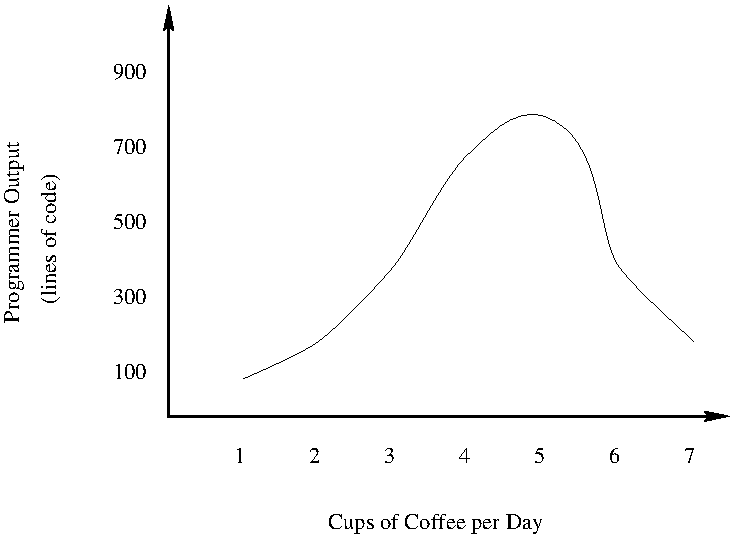
\includegraphics[width = 100mm]{graph1.pdf}
\caption[Another example of a floating figure.]{This figure has been
forced into position by using the [!h] option.}
\label{fig:graph2}
\end{center}
\end{figure}

Figure~\ref{fig:graph2} has been placed right where it is included in
the document, using the [!h] instead of [htb].  If [!h] is not strong
enough, it can be made even stronger by using the [H] option.

You can also scale figures based on their original sizes;
Figure~\ref{fig:graph3} has been scaled by a factor of 50\% using the
option [scale = 0.5].

\begin{figure}[!h]
\begin{center}
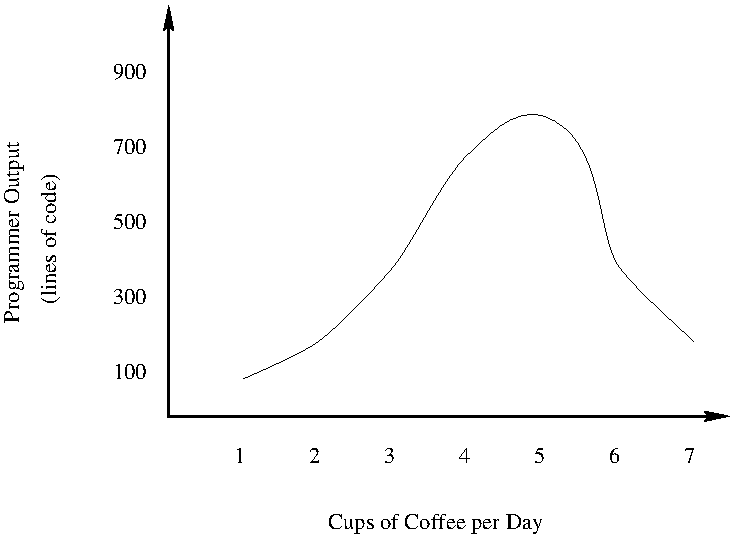
\includegraphics[scale = 0.5]{graph1.pdf}
\caption[A scaled example of a floating figure.]{This figure has been
been scaled from its original size.}
\label{fig:graph3}
\end{center}
\end{figure}

This is one of the most obvious reasons to use PDF
graphics when creating diagrams---PDF vector diagrams will scale
perfectly and print out crisply and 
clearly, with no ``jaggies''.  Just about every graphics program in
common use will output PDF graphics for you.

If you use GNU programs like {\tt xfig}, {\tt dia} or {\tt gimp} to do
your diagrams or screen-shots, you will have no problem exporting files as
PDF.

Figure~\ref{fig:page} is an example of the point above.  It is
the contents page of this very document; first, the document was
compiled by typing {\tt make}.  Next, the contents page was viewed
using {\tt gv} and saved as a separate PDF file.  It was
rotated about \(90^\circ\) by using the [angle=90] option in the
\verb|\includegraphics| command.

\begin{figure}[tb]
\begin{center}
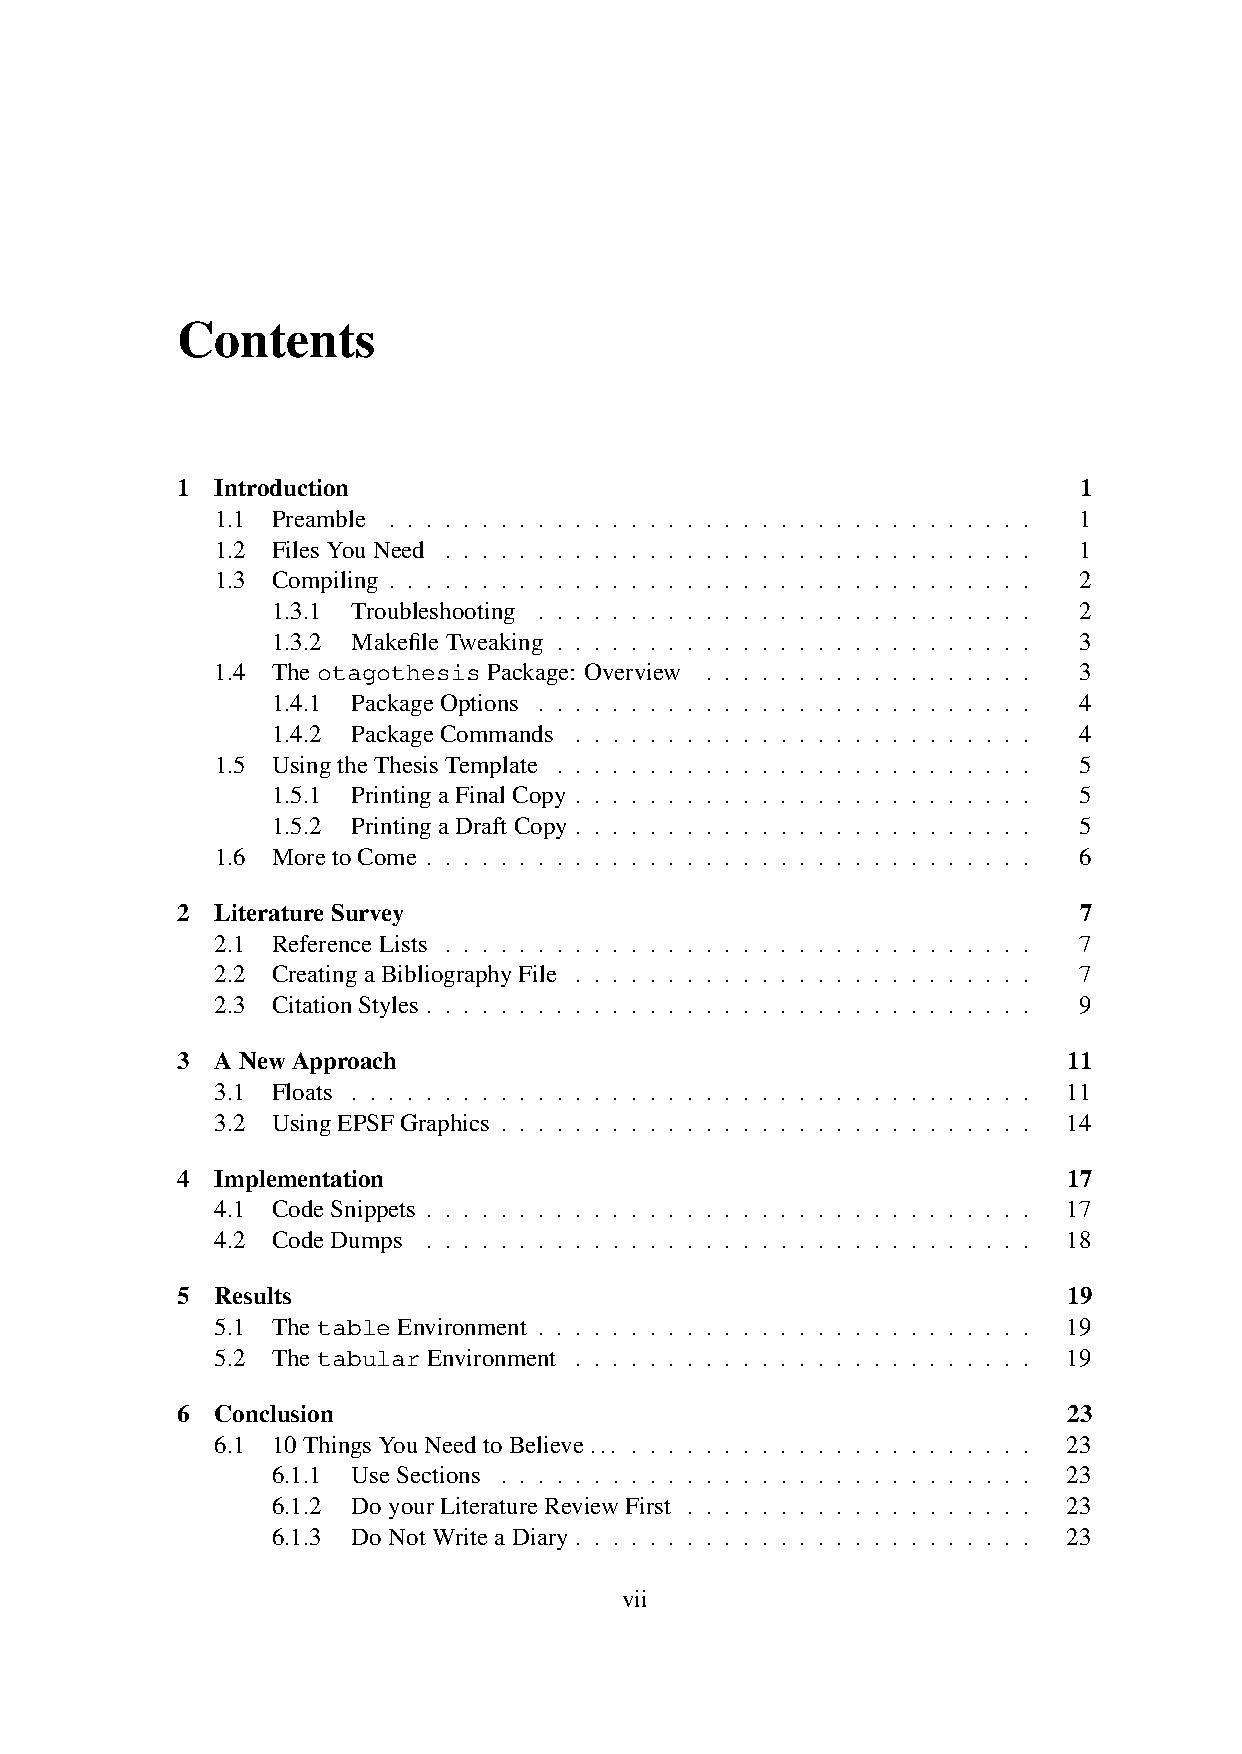
\includegraphics[scale = 0.6, angle = 90]{page.pdf}
\caption[A PDF page included as a figure.]{This is the contents
page of this document, included as a floating figure and scaled to
60\% of its original size}
\label{fig:page}
\end{center}
\end{figure}

The \verb|otagothesis| Makefile has a feature especially for xfig
users.  If you uncomment the line that starts with the word
\verb|FIGFILES|, put your xfig figures in the same directory as
your thesis, and put their filenames in place of
\verb|ex1.fig ex2.fig| etc., the Makefile will call \verb|fig2dev| on
them to convert them all to pdf format.  As a result, you don't have
to export your figures from xfig as pdf; just save them as regular
\verb|.fig| format in your thesis directory.  NOTE: this requires
installation of the \verb|xfig/fig2dev| software on MacOsX.

A final word about figures, from \citet[p141 ff]{goosens94}:
\begin{quotation}
Floats are often problematical in the present version of \LaTeX,
since the system was developed at a time when the amount of graphical
material in a document was considerably less than it is now \ldots\
If \ldots\ a lot of floating material is present \ldots\ then it is often
the case that all material from a certain point onwards floats to the
end of the document.
\end{quotation}
In fact, this can cause a real problem---not only is it ugly, but if
too many floats remain unprocessed before the end of the document is
reached, \LaTeX\ will die with a ``too many unprocessed floats'' error.
This can be fixed by periodically issuing the command
\verb|\clearpage|, which forces all as-yet unprocessed floats to be
printed.
